\DomainHeader{Data Modeling}{13\%}

\begin{Objectives}
  \item Add a primvar to a mesh.
  \item Choose correct value types for attribute data.
  \item Represent custom metadata.
  \item Retrieve properties of a prim.
  \item Diagnose causes of unexpected visual results.
  \item Update \texttt{extent} after updating \texttt{points}.
\end{Objectives}

\begin{Resources}
  \item Learn OpenUSD: Setting the Stage; Scene Description Blueprints; Beyond
        the Basics
  \item User guide: Rendering --- Working With Primvars
  \item OpenUSD glossary: TimeCode; Layer Offset; List Editing; Primvar
  \item OpenUSD API: Sdf datatypes; UsdGeomPrimvar; Boundable; XformCache;
        UsdAttribute interpolation
\end{Resources}

\CheatSheetTitle
\begin{itemize}[leftmargin=*]
  \item \textbf{Two property kinds}: \emph{attributes} carry typed values
        (defaults + time samples); \emph{relationships} carry targets (paths).
        \index{attribute}\index{relationship}
  \item \textbf{Metadata is not an attribute}: it hangs on prims, properties,
        layers, or the stage; it is \emph{never} time-sampled
        (\texttt{kind}, \texttt{assetInfo}, \texttt{customData}).\index{metadata}
  \item \textbf{Primvars} are namespaced attributes (\texttt{primvars:*}) with
        an \emph{interpolation}: constant, uniform (per face), vertex,
        faceVarying --- and optional \texttt{:indices}.\index{primvar}
  \item \textbf{Value types carry meaning}: \texttt{color3f} vs
        \texttt{point3f} vs \texttt{normal3f} vs \texttt{vector3f} are all
        three floats --- the \emph{role} drives transformation and color
        handling.
  \item \textbf{token} for closed vocabularies, \texttt{string} for text,
        \texttt{asset} for paths, \texttt{rel} for ``points at another prim''.
  \item \textbf{extent is data}: bounds are authored; whoever moves
        \texttt{points} must re-author \texttt{extent}.\index{extent}
  \item \textbf{Visual surprises} are usually data: interpolation/count
        mismatch, stale extent, wrong role type, or indices out of range.
\end{itemize}

\section{Core Concepts}

\subsection{The property taxonomy}\label{sec:dm-tax}\objref{5.4}

\begin{figure}[ht]
  \centering
  \begin{tikzpicture}[node distance=3mm and 6mm]
    \node[primbox, minimum width=2.8cm] (prop) {Property};
    \node[primbox, minimum width=3.2cm, below left=8mm and 2mm of prop] (attr) {Attribute};
    \node[primbox, minimum width=3.2cm, below right=8mm and 2mm of prop] (rel) {Relationship};
    \node[notetext, below=1mm of attr, align=center]
      {typed values\\defaults + time samples\\(\texttt{primvars:*} included)};
    \node[notetext, below=1mm of rel, align=center]
      {targets: prim/property paths\\(\texttt{material:binding}, proto lists)};
    \node[layerbox, right=18mm of prop, minimum width=2.8cm] (meta) {Metadata};
    \node[notetext, below=1mm of meta, align=center]
      {on prims, properties, layers\\never time-sampled};
    \draw[arc, draw=black!55] (prop.south) -- (attr.north);
    \draw[arc, draw=black!55] (prop.south) -- (rel.north);
  \end{tikzpicture}
  \caption{What can hold data in USD. The exam loves the boundaries: a
  time-varying value can never live in metadata; a path target can never live
  in an attribute.}
  \label{fig:prop-taxonomy}
\end{figure}

\subsection{Value types and roles}\label{sec:dm-types}\objref{5.2}
Sdf's type registry pairs storage with \emph{role}. Choosing well is an exam
objective in itself:

\begin{lstlisting}
#usda 1.0
( defaultPrim = "Props" )
def Scope "Props" {
    def Xform "Crate" {
        token visibility = "inherited"
        asset texture = @./wood.png@
        color3f[] primvars:displayColor = [(0.4, 0.25, 0.1)]
        matrix4d xformOp:transform = ( (1, 0, 0, 0), (0, 1, 0, 0),
                                       (0, 0, 1, 0), (0, 0, 0, 1) )
        uniform token[] xformOpOrder = ["xformOp:transform"]
        custom string notes = "hero prop"
        custom rel inspiration = </Props/Reference>
    }
    def Xform "Reference" {
    }
}
\end{lstlisting}

\noindent\texttt{token} is for closed vocabularies the runtime switches on
(\texttt{visibility} values); \texttt{asset} marks resolver-relevant paths;
the \texttt{color3f}, \texttt{point3f}, \texttt{normal3f}, and
\texttt{vector3f} roles tell consumers how to transform and color-manage
three floats;
\texttt{uniform} means ``not time-sampleable''; and a relationship ---
\texttt{rel} --- is the only correct way to say ``that prim over there''.
Figure~\ref{fig:propspanel} is this exact prim in usdview's property panel.

\begin{figure}[ht]
  \centering
  \begin{tikzpicture}
    \node[anchor=south west, inner sep=0] (img)
      {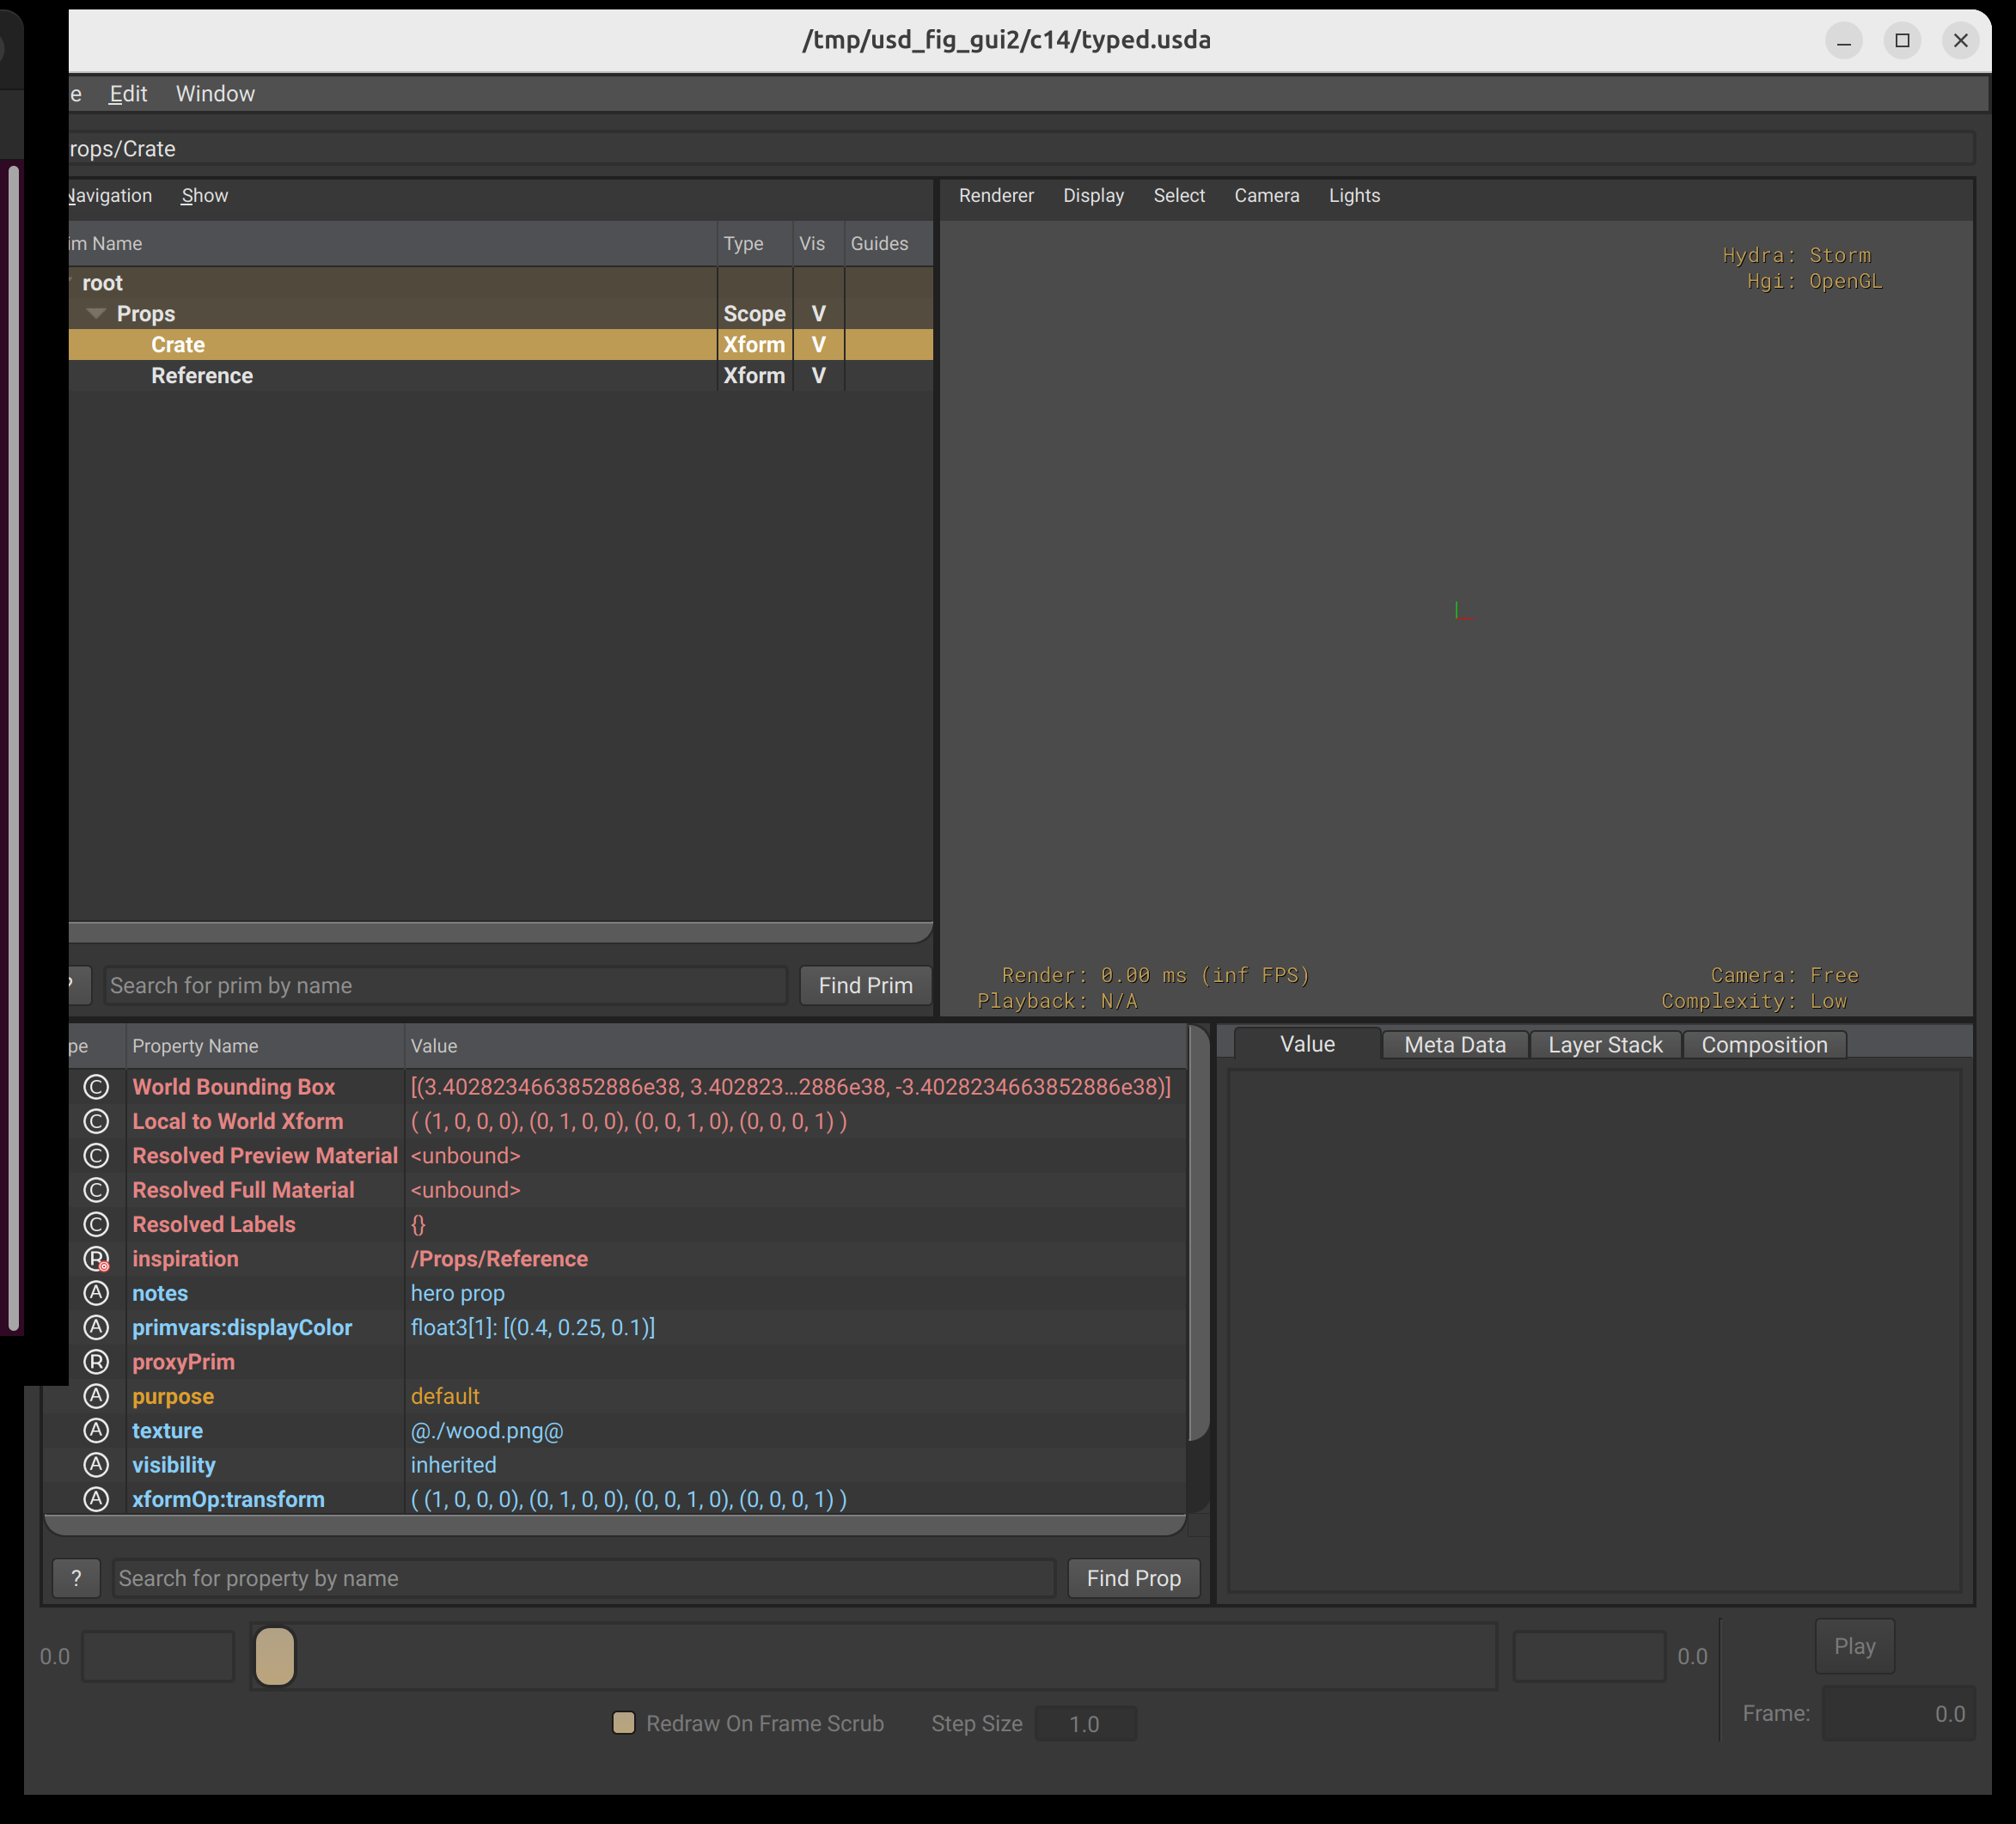
\includegraphics[trim={30 0 0 0}, clip, width=0.95\linewidth]{figures/c14_usdview_props.png}};
    \begin{scope}[x={(img.south east)}, y={(img.north west)}]
      \node[notetext, draw=arcRef, fill=white, rounded corners=1pt,
            text width=0.27\linewidth, align=left] (rel) at (0.74,0.37)
        {a relationship's ``value'' is a target path};
      \draw[refArc] (rel.west) -- (0.36,0.315);
      \node[notetext, draw=arcPay!85!black, fill=white, rounded corners=1pt,
            text width=0.27\linewidth, align=left] (ast) at (0.74,0.20)
        {asset-typed: quoted with \texttt{@...@}, visible to the resolver};
      \draw[payArc] (ast.west) -- (0.33,0.225);
    \end{scope}
  \end{tikzpicture}
  \caption{The type-zoo prim in usdview: every property displays its declared
  type and role --- \texttt{inspiration} resolves to a prim path,
  \texttt{texture} to an asset path, \texttt{primvars:displayColor} to a
  color array. Property retrieval, made visual.}
  \label{fig:propspanel}
\end{figure}

\subsection{Primvars and interpolation}\label{sec:dm-primvars}\objref{5.1, 8.1}
\index{primvar}\index{interpolation}A primvar is an attribute in the
\texttt{primvars:} namespace plus two superpowers: it \emph{inherits down
namespace} (constant primvars flow to descendants) and it carries
\emph{interpolation} --- how values map onto the surface:

\begin{lstlisting}
#usda 1.0
( defaultPrim = "Plate" )
def Mesh "Plate" {
    float3[] extent = [(-1, 0, -1), (1, 0, 1)]
    int[] faceVertexCounts = [4]
    int[] faceVertexIndices = [0, 1, 2, 3]
    point3f[] points = [(-1, 0, -1), (1, 0, -1), (1, 0, 1), (-1, 0, 1)]
    texCoord2f[] primvars:st = [(0, 0), (1, 0), (1, 1), (0, 1)] (
        interpolation = "faceVarying"
    )
    int[] primvars:st:indices = [0, 1, 2, 3]
}
\end{lstlisting}

\noindent Element-count rules: \emph{constant} = 1, \emph{uniform} = one per
face, \emph{vertex} = one per point, \emph{faceVarying} = one per
face-vertex (corner) --- with \texttt{:indices}, the rule applies to the
\emph{indices}, letting corners share values. UVs are typically
\texttt{primvars:st}, faceVarying, indexed.

\begin{Gotcha}
\objref{5.5, 6.4}``My render looks wrong'' is usually one of: interpolation whose element
count does not match the data (validator material!), \texttt{:indices}
pointing past the value array, a \texttt{vector3f} treated as a
\texttt{point3f} (translations apply to points, not vectors), or a stale
\texttt{extent} culling the mesh. All four are data bugs, not renderer bugs.
\end{Gotcha}

\subsection{Authoring and retrieving with the API}\label{sec:dm-api}\objref{5.1, 5.3, 5.4}
The same model drives the Python surface --- create a primvar, stash custom
metadata, list what a prim carries:

\begin{lstlisting}[language=Python]
from pxr import Sdf, Usd, UsdGeom

stage = Usd.Stage.CreateInMemory()
mesh = UsdGeom.Mesh.Define(stage, "/Crate")
prim = mesh.GetPrim()

wear = UsdGeom.PrimvarsAPI(prim).CreatePrimvar(
    "wear", Sdf.ValueTypeNames.Float, UsdGeom.Tokens.constant)
wear.Set(0.5)

prim.SetCustomDataByKey("studio:reviewed", True)

print(wear.GetName(), wear.Get(), wear.GetInterpolation())
# primvars:wear 0.5 constant
print(prim.GetCustomDataByKey("studio:reviewed"))   # True
print([a.GetName() for a in prim.GetAttributes() if a.IsAuthored()])
# ['primvars:wear']
\end{lstlisting}

\noindent Retrieval comes in layers of specificity:
\texttt{GetPropertyNames()} (everything), \texttt{GetAttributes()} /
\texttt{GetRelationships()} (by property kind),
\texttt{GetPropertiesInNamespace("primvars")} (by namespace), and schema
accessors (\texttt{GetPointsAttr()}) when you know the type.\index{customData}

\begin{ExamTip}
\texttt{customData} is the junk drawer --- free-form, ignored by the runtime.
\texttt{assetInfo} is for asset identity. If the data needs a \emph{type},
\emph{time samples}, or \emph{querying at scale}, it wants to be an
attribute (or a proper schema), not metadata.
\end{ExamTip}

\subsection{Keeping extent honest}\label{sec:dm-extent}\objref{5.6}
\index{extent}Whoever updates \texttt{points} owns \texttt{extent} --- the
exam states it as its own objective, and Sample Question 5 tests it:

\begin{lstlisting}[language=Python]
from pxr import Usd, UsdGeom

stage = Usd.Stage.Open("mesh_uv.usda")
mesh = UsdGeom.Mesh(stage.GetPrimAtPath("/Plate"))

points = [(x * 2, y * 2, z * 2) for x, y, z in mesh.GetPointsAttr().Get()]
mesh.GetPointsAttr().Set(points)

extent = UsdGeom.Boundable.ComputeExtentFromPlugins(
    mesh, Usd.TimeCode.Default())
mesh.GetExtentAttr().Set(extent)
print(extent)   # [(-2, 0, -2), (2, 0, 2)]
\end{lstlisting}

\subsection{Time, samples, and interpolation}\label{sec:dm-time}\objref{5.2, 5.5}
\index{timeSamples}\index{TimeCode}An attribute holds a \emph{default} and
optionally \emph{time samples}; queries take a \texttt{TimeCode}:

\begin{lstlisting}
#usda 1.0
( defaultPrim = "Ball" )
def Sphere "Ball" {
    double radius.timeSamples = {
        1: 1,
        11: 11,
    }
}
\end{lstlisting}

\begin{lstlisting}[language=Python]
from pxr import Usd

stage = Usd.Stage.Open("ball_anim.usda")
radius = stage.GetPrimAtPath("/Ball").GetAttribute("radius")

print(radius.Get(6))                       # 6.0  -- linear interpolation
print(radius.GetBracketingTimeSamples(6))  # (1.0, 11.0)

stage.SetInterpolationType(Usd.InterpolationTypeHeld)
print(radius.Get(6))                       # 1.0  -- held: previous sample
\end{lstlisting}

\noindent Three rules cover most exam traps: between samples, the
\emph{stage's} interpolation type decides (linear by default, held as an
option --- there is no spline yet); outside the sampled range the nearest
sample is held; and \texttt{Get()} with no argument means
\texttt{TimeCode.Default()}, which reads the \emph{default value, not the
samples} --- an attribute with only time samples returns nothing at Default.

\begin{Gotcha}
``The value is right in usdview but wrong in my script'' is often a
\texttt{TimeCode} bug: usdview queries at the current frame; your script
queried Default. Pass the time explicitly ---
\texttt{attr.Get(Usd.TimeCode(frame))} --- whenever samples exist.
\end{Gotcha}

\subsection{Transforms without tears: XformCommonAPI}\label{sec:dm-xform}\objref{5.1, 5.4}
\index{XformCommonAPI}\index{xformOp}Raw \texttt{xformOp:*} attributes are
flexible and easy to get wrong (op order!). For the standard
translate/rotate/scale case, \texttt{XformCommonAPI} authors a canonical
stack and reads it back as plain vectors:

\begin{lstlisting}[language=Python]
from pxr import Gf, Usd, UsdGeom

stage = Usd.Stage.CreateInMemory()
prim = UsdGeom.Xform.Define(stage, "/Crate").GetPrim()

api = UsdGeom.XformCommonAPI(prim)
api.SetTranslate(Gf.Vec3d(1, 2, 3))
api.SetRotate(Gf.Vec3f(0, 45, 0))
api.SetScale(Gf.Vec3f(2, 2, 2))

t, r, s, pivot, order = api.GetXformVectors(Usd.TimeCode.Default())
print(t, r, s)   # (1, 2, 3) (0, 45, 0) (2, 2, 2)
\end{lstlisting}

\noindent For world-space answers across a hierarchy, use
\texttt{UsdGeom.XformCache} --- it memoizes local-to-world matrices per time
code, which is also the right tool inside exporters.\index{XformCache}

\DrillsTitle
\subsection*{Drill 1: Primvar practice}
Write a minimal Mesh that includes \texttt{primvars:st} with faceVarying
interpolation.
\AnswerLines{10}
\begin{DrillSolution}
The chapter's Plate listing is the reference answer: counts/indices/points
for one quad, \texttt{texCoord2f[] primvars:st} with
\texttt{interpolation = "faceVarying"} in the attribute metadata, plus
\texttt{primvars:st:indices} so corners can share values. Bonus points in an
exam answer: authored \texttt{extent}.
\end{DrillSolution}

\subsection*{Drill 2: Type discipline}
Give 6 examples of common types (token, rel, float3, color3f[], matrix4d,
asset) and what you'd store in them.
\AnswerLines{8}
\begin{DrillSolution}
\texttt{token} --- closed vocabulary like \texttt{purpose = "proxy"};
\texttt{rel} --- ``points at'' data like \texttt{material:binding};
\texttt{float3}/\texttt{point3f}/\texttt{vector3f} --- positions vs
directions (role matters under transforms); \texttt{color3f[]} ---
\texttt{primvars:displayColor}; \texttt{matrix4d} ---
\texttt{xformOp:transform}; \texttt{asset} --- texture and layer paths the
resolver should see (never plain strings).
\end{DrillSolution}

\subsection*{Drill 3: Element-count audit}
A quad mesh (4 points, 1 face, 4 corners) has primvars with 1, 4, and 4
values. Which interpolations are legal for each?
\AnswerLines{6}
\begin{DrillSolution}
1 value $\Rightarrow$ constant. 4 values $\Rightarrow$ vertex (per point)
\emph{or} faceVarying (per corner --- this quad has exactly 4 corners), so
both are legal here; the distinction starts to matter the moment two faces
share a point. 4 values can never be uniform on a 1-face mesh (uniform needs
exactly 1).
\end{DrillSolution}

\section*{Checkpoint Questions}
\addcontentsline{toc}{section}{Checkpoint Questions}

\noindent\textbf{CQ1.} Where can a time-varying review note live: attribute
metadata, \texttt{customData}, or an attribute --- and why?
\begin{DrillSolution}
Only an attribute --- metadata (including \texttt{customData}) is never
time-sampled. If it varies over time, it is a value, and values live in
attributes.
\end{DrillSolution}

\noindent\textbf{CQ2.} \texttt{primvars:st} has 4 values,
\texttt{interpolation = "vertex"}, on a mesh with 6 points. What happens?
\begin{DrillSolution}
Element-count mismatch: vertex interpolation requires one value per point
(6). Renderers may drop the primvar, render garbage UVs, or warn --- the
asset is invalid even though it parses. This is exactly the class of
``unexpected visual results'' the exam asks you to diagnose.
\end{DrillSolution}

\noindent\textbf{CQ3.} After a tool doubles all \texttt{points}, the mesh
disappears in some views. Likely cause and fix?
\begin{DrillSolution}
Stale \texttt{extent}: bounds still describe the old size, so the camera or
renderer culls incorrectly. Recompute with
\texttt{ComputeExtentFromPlugins} and re-author \texttt{extent} --- the
chapter's listing is the fix, verbatim.
\end{DrillSolution}

\subsection*{Mini-checklist (tick when mastered)}
\begin{itemize}[leftmargin=*]
  \item[$\square$] I can place any datum: attribute vs relationship vs metadata.
  \item[$\square$] I can recite the four interpolations and their element counts.
  \item[$\square$] I know when \texttt{:indices} applies and what it changes.
  \item[$\square$] I re-author \texttt{extent} reflexively after touching \texttt{points}.
\end{itemize}
